\documentclass[tikz,border=14pt]{standalone}
\usepackage{amsmath,amssymb}
\usetikzlibrary{arrows.meta}
\definecolor{ink}{HTML}{E4EDF8}
\definecolor{muted}{HTML}{596B80}
\definecolor{blue}{HTML}{9FC2FF}
\definecolor{teal}{HTML}{63D3BB}
\definecolor{gold}{HTML}{E7C274}
\definecolor{panel}{HTML}{111923}
\pagecolor{panel}
\color{ink}
\begin{document}
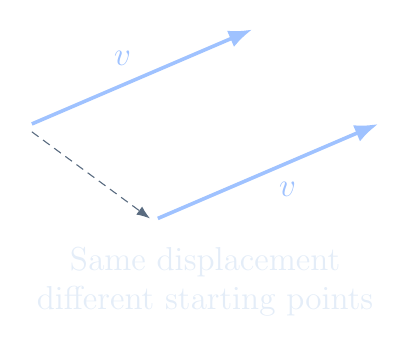
\begin{tikzpicture}[font=\large,text=ink,vec/.style={-{Latex[length=3mm]},line width=1.3pt},axis/.style={muted,-{Latex[length=2mm]},thin}]
\draw[vec,blue] (0,0)--(2.8,1.2) node[midway,above left] {$v$};
\draw[vec,blue] (1.6,-1.2)--(4.4,0) node[midway,below right] {$v$};
\draw[densely dashed,muted,-{Latex}] (0,-.1)--(1.5,-1.2);
\node[align=center,text=ink] at (2.2,-2) {Same displacement\\different starting points};
\end{tikzpicture}
\end{document}
